\subsection{نظرة عامة}



\subsection{الأدوات}
\subsubsection{التغذية الراجعة}
إنّ تحديد نظام التّغذية الرّاجعة (XYTheta feedback) كان الخطوة الأساسيّة لنا لوضع تصوّر أساسي للمشروع ولبدء عمليّة التّصميم واختيار القطع الإلكترونيّة بحيث نحصل على أفضل أداء ممكن وفق تصميم مناسب وأسعار مقبولة. اعتمدنا في هذه المرحلة على نظام نقاط بين 1 و 5 - حيث يشير الرّقم 5 إلى الأفضليّة العليا – للمفاضلة بين الخيارات المتاحة وفق معايير محدّدة كما هو موضّح في الجدول أدناه.

\begin{table}[h]
	\begin{tabular}{lccccccc|}
		\cline{2-8}
	\multicolumn{1}{l|}{} & الحاجة للاختبار  &  فعالية التحكم & سهولة التطبيق & سهولة التصميم  & الحاجة  & السعر &    \\ \hline
		\multicolumn{1}{|l}{Dead Reckoner} & 3 & 4 & 4 & 5 & 3 & 5 & 24 \\ \hline
		\multicolumn{1}{|l}{Mouse Sensor}  & 1 & 5 & 2 & 3 & 5 & 4 & 20 \\ \hline
		\multicolumn{1}{|l}{Camera}        & 5 & 5 & 2 & 5 & 3 & 5 & 25 \\ \hline
	\end{tabular}
\end{table}


بعد عمليّة المقارنة وبناءً على النّتائج الموضّحة أعلاه كان خيار استخراج مواقع الرّوبوتات من كاميرا مثبّتة فوق حلبة عمل الرّوبوتات هو الخيار الأفضل. 
أمّا عمليّة اختيار الكاميرا فكانت ترتكز على معيارين أساسين وهما الحصول على تغطية كاملة للمنّصة و عدد الأطر التي يمكن الحصول عليها في الثّانية الواحدة. لذلك قمنا باختيار كاميرا ستريو واسعة الزّاوية الّتي تعدّ خياراً مناسبا لنا. حيث أنّ  أبعاد حساس كل كاميرا 960×2560 بكسل. يمكن بسهولة إيجاد أنّ أصغر مسافة يمكن قياسها باستخدام الكاميرا عن طريق تقسيم عرض فضاء العمل ( على دقة حسّاس الكاميرا و النتيجة هي 2.5 mm. بالإضافة إلى إمكانيّة الحصول على 16 إطار بالثّانية وهو تردّد كافٍ لمتابعة سير الروبوتات وتحديد مواقعها.

\subsubsection{المحرك}
المعايير الأساسيّة الّتي تمّ اعتمادها لاختيار المحركات: طريقة قياس لموضع وطريقة قيادة الرّوبوت ولقد اعتمدنا لتحديد ذلك النّظام النّقطي السّابق الّذي اعتمدناه لتحديد نظام التّغذية الرّاجعة في الفقرة السّابقة.

\begin{table}[h]
	\begin{tabular}{lccccccc|}
		\cline{2-8}
		\multicolumn{1}{l|}{} & الحاجة للاختبار  &  فعالية التحكم & سهولة التطبيق & سهولة التصميم  & الحاجة  & السعر &    \\ \hline
		\multicolumn{1}{|l}{ODD BLDC} & 1 & 5 & 1 & 1 & 3 & 4 & 15 \\ \hline
		\multicolumn{1}{|l}{Micro Servo}  & 5 & 3 & 5 & 5 & 3 & 1 & 22 \\ \hline
		\multicolumn{1}{|l}{Gear DC}        & 2 & 4 & 1 & 1 & 2 & 3 & 13 \\ \hline
	\end{tabular}
\end{table}


كما نرى في الجدول السّابق فإنّ محرّك الـ Micro servo كان الخيار الأكثر ملائمة ولاسيّما مع سهولة استخدامه وتغليفه الّذي سوف يسهّل عمليّة التّصميم بشكل كبير  بالإضافة إلى سعره المقبول. ولكنّه كان بحاجة لعمليّة اختبار للتأكد من مدى قدرتنا على التّحكم به و عن مدى قدرتنا على التّحكم به. لذلك قمنا باالتّجريب على محرك SG90 Continuous 360 Degree. يبلغ وزن المحرك 9 غرام وعزمه عند جهد تغذية 4.8 فولت $1.3 Kg.cm$ وسرعة الدوران الأعظمية 110 دورة في الدقيقة.

لكنّ نتائج الاختبار لم تكن مرضية بشكل كامل؛ حيث بينت الاختبارات وجود منطقة ميتة في خرج الاكودر الداخلي للمحرك dead band. لكنّ الخيارات الاخرى كانت غير مناسبة من ناحية التّوافر؛ لذلك لجأنا إلى حل آخر، وهو فصل محرّك التّيار المستمرّ الموجود داخل الـ SG90  عن دارة قيادته ووصله مع المقاومة المتغيّرة الدّاخلية إلى دراتنا السفليّة و باالتّالي يمكن استخدام محرّكات تيّار مستمرّ بحجم مناسب وضمن تغليف مناسب مّما سهّل علينا عمليّة تصميم الجسم وتصغير حجمه بالإضافة إلى السّعر المناسب. كما أنّنا سوف نقوم باستخدام العجلات كمسجلّات للحركة من أجل تحكّم أكثر دقّة.

\subsubsection*{قيادة المحرك}
 بالنّسبة لقيادة محركات التيار المستمر، فتم ذلك باستخدام الجسر L298. يعاني الجسر من عدة مشاكل أهمها قدم تكنولوجيا TTL المستخدمة في صناعته، وأيضاً كبر حجمه. ممّا فرض قيوداً في الحجم والشّكل على تصميم الدّارات  لذلك استخدمنا L298N - Dual Full-Bridge Driver IC وسنرى لاحقا كيف أنّ تصميم الدّارات وتجميعها مكّننا من تنفيذ الشروط المطلوبة للتّصميم ضمن القيود المفروضة عليه.
 
\subsection{وحدة التحكم}
لتغطية كافة احتياجات النظام الإلكتروني تمّ وضع عدة نقاط رئيسية يجب على النظام المدمج في الروبوت شملها:

\begin{itemize}
	\item اتصال آمن وبتأخير (latency) منخفضة بين الروبوت والنظام المركزي.
	\item القدرة على قيادة محركي DC بجهد أعظمي 7.5 v وتيار 0.5 A أعظمي.
	\item عرض نبضة بتردد متوافق من الثابت الزمني للمحرك.
	\item نظام تحديد سرعة وموضع كل من محركي التيار المستمر.
	\item نظام تغذية.
	\item وحدات ادخال وإخراج بدائية بغية الـdebugging وتبديل البارامترات الداخلية on-the-run.
\end{itemize}

اعتمدنا على سلسلة متحكمات الـ 8 bit الخاصة بشركة Atmel ذات الـInstruction set RISC. يوجد في هذه المتحكمات 35 تعليمة بالإضافة لعدة وحدات توقيت ومقاطعات داخلية وخارجية تجعل المهمة المطلوبة ممكنة. ولقد اخترنا المتحكّم  Atmega328p tqfp.

يمتلك المتحكم Atmega328p المواصفات الآتية:
\begin{english}
\begin{itemize}
	\item Two 8-bit Timer/Counter
	\item One 16-bit Timer/Counter
	\item UART Connection Unit
	\item Two External Interrupt Unit
	\item I2C Unit
	\item Three 8-bit I/O units
	\item One ADC Unit with MUX to 8-bit I/O Unit
\end{itemize}
\end{english}


يضمن وجود ثلاث مؤقتات/عدادات قدرة النظام على جدولة المهام حسب أولوياتها وحسب الوقت المطلوب لها. كما انها توفر العتاد المطلوب لتشكيل إشارة بعرض نبضة متغير PWM تستخدم لقيادة محركات التيار المستمر. (يتم تشكيلها باستخدام الـHardware). توفر وحدة الـUART الاتصال المباشر بين وحدة الاتصال وبين المتحكم وبشكل سهل ومباشر وآمن من الأخطاء. أما بالنسبة للمقاطعات الخارجية: فهي تسمح للمتحكم بتسجيل الحركة التي تسجلها المقاطعات الضوئية المستخدمة في قراءة دوران المحرك.

\subsection{التغذية}

باختلاف التّصورات المحتملة لسرب الرّوبوتات، فإنّ كل روبوت ضمن السّرب يحتاج إلى إمداده بطاقة لإكمال المهمّة الموكلة له. ولقد قمنا باختيار بطّاريات  Lithium-Ion القابلة لإعادة الشّحن؛ حيث يمكن إعادة شحن هذا النّوع من البّطاريات مئات المرّات مع الحفاظ على ثباتها وأدائها مقارنةً بغيرها من البطّاريات. تميل بطّاريات Lithium-Ion إلى أن تكون ذات كثافة طاقة أعلى، معدّل تفريغ ذاتي أقلّ من البطّاريات الأخرى القابلة لإعادة الشّحن؛ ممّا يؤدّي إلى تحسين كفاءة الطاقة حيث تتمتّع الخليّة الواحدة باحتفاظ بالشّحن لفترة أطول من أنواع البطّاريات الأخرى. أمّا بالنّسبة للشكل: فلقد اخترنا بطاريات بأبعاد ( 4 mm× 4 cm ×5 cm ) لكي تتناسب مع التّصميم. وتقدّم هذه البطّاريات جهداً مقداره 3.7 V وتتوضّع عليها دارة حماية.

إنّ استخدام مصدر تغذية قابل لإعادة الشّحن يفرض علينا استخدام وحدة شحن وتفريغ. ولقد استخدمنا وحدات TP4056A المستخدمة لشحن وتفريغ بطّاريات اللّيثوم أيّون. ونظراً إلى أنّ البطّاريّات المستخدمة تقدّم جهد 3.7 V؛ احتجنا إلى استخدام وحدة رافع جهد (DC- DC convertor). إنّ دخل دارة رافع الجهد يتراوح بين 3 إلى 15 فولت، بينما يكون الخرج من 4 إلى 35 فولت، ويتمّ ضبطها لإعطاء الخرج المطلوب بشكل يدوي.


\subsection{نظام الاتصال}
بعد قراءة الدّراسات المرجعيّة واستشارة المختصّين تم اعتماد تقنية الواي فاي لربط الروبوتات مع بعضها ومع الحاسوب المركزي. ولاختيار وحدة الواي فاي المناسبة.
% Please add the following required packages to your document preamble:
% \usepackage{multirow}
\begin{table}[h]
	\resizebox{\textwidth}{!}{\begin{tabular}{lrccccc|}
			\cline{3-7}
			\multicolumn{2}{l}{\multirow{2}{*}{}}                                                                                                               & \multicolumn{2}{|c|}{\textbf{وحدات   بدائية}}       & \multicolumn{3}{c|}{\textbf{وحدات   مطوّرة}}                                \\ \cline{3-7} 
			\multicolumn{2}{l}{}                                                                                                                                & \multicolumn{1}{|c}{ESP-01}              & ESP-12e             & NodeMcu-DevKit-V1.0 & NodeMcu-Lua-WIFI-Board & Wemos-D1-Mini       \\ \hline
			\multicolumn{1}{|l|}{المداخل   والمخارج للأغراض العامّة} & GPIO & 2                   & 11                  & 11                  & 11                     & 11                  \\ \hline
			\multicolumn{1}{|l|}{محوّل   تماثلي رقمي}                & ADC       & -                   & 1                   & 1                   & 1                      & 1                   \\ \hline
			\multicolumn{1}{|l|}{هوائي}                              & Antenna                                                                                  & مطبوعة   على الدارة & مطبوعة   على الدارة & مطبوعة   على الدارة & مطبوعة   على الدارة    & مطبوعة   على الدارة \\ \hline
			\multicolumn{1}{|l|}{إمكانيّة   الوصل المباشر}           & USB-to-Serial                                                                            & غير ممكن            & غير ممكن            & ممكن                & ممكن                   & ممكن                \\ \hline
			\multicolumn{1}{|l|}{عامل   الشّكل}                      & Form                                                                              & صغير                & متوسط               & كبير                & كبير                   & متوسط               \\ \hline
			\multicolumn{1}{|l|}{وحدة الـ  ESP8266}                  & ESP8266 Module                                                                           & -                   & -                   & ESP12E & ESP12E   & ESP12E       \\ \hline
			\multicolumn{1}{|l|}{شريحة   الوصل المباشر}              & Serial                                                                              & -                   & -                   & CH340G              & CP2102                 & CH340G              \\ \hline
			\multicolumn{1}{|l|}{غطاء لحجب   التّرددات الرّاديويّة}  & RF-shield                                                                             & لايوجد              & يوجد                & يوجد                & يوجد                   & يوجد                \\ \hline
	\end{tabular}}
	\label{table::rfmodule}
	\caption{جدول مقارنة بين وحدات الاتصال المختلفة}
\end{table}

وتم التقييم وفق معايير معينة وهي الوثوقية، الحجم، التوافرية، السعر، وامكانية الوصل المباشر (USB-to-Serial) . بناءً على هذه المعايير والجدول السّابق قمنا باختيار وحدة الاتّصال Wemos  ؛ حيث أنّها تحقق ذات وثثوقيّة عالية مقارنة بسعرها وحجمها مناسب بالإضافة إلى توافرها.

\subsection{الدارة الالكترونية المطبوعة PCB}

يتم قيادة محرك التيار المستمر باستخدام الجسر L298. يعاني الجسر من عدة مشاكل أهمها قدم تكنولوجيا TTL المستخدمة في صناعته، وأيضاً كبر حجمه. ممّا فرض قيوداً في الحجم والشّكل على تصميم الدّارات. سوف نعرض في الفقرتين التاليتين تجميعة الدارات التي مكنتنا من تنفيذ الشروط السابقة ضمن قيود الحجم والشكل المفروضة عليه. حيث سنقوم في القسم الأول بشرح عملية تصميم أمّا في القسم الثّاني سوف نقوم باستعراض عمليّة التّصنيع.

\subsubsection{التصميم باستخدام الحاسب}
لقد استخدمنا البرنامج التّصميمي Altium لتصميم الطّبقة العلويّة والسفليّة. حيث أن الطّبقة العلويّة تحتوي على وحدة الاتصال والمتحكّم الصغري ووحدات الادخال والإخراج، بينما يحتوي يضم القسم السّفلي جسر القيادة، وحدات التغذية وشحن المدخرة، ودارات المقطعات الضوئية. 

\subsubsection*{الطبقة العلوية:  طبقة المعالجة والإشارة}
 هذه الطبقة مسؤولة عن أي اجراء على الروبوت القيام به حسابياً أو لتلقي أوامر الحركة من حاسوب مركزي. تحوي الطبقة متحكمين اثنين: الأول بمعمارية RISC AVR 8 bit والثاني 32-bit. يوفر المعالج الأول الوسائل المنطقية والتوقيتية للتحكم بالمحركات بدقة وكذلك لإجراء حسابات المعادلات الفروقية بدور تقطيع بالغ الدقة، أي للقيادة منخفضة المستوى. أما المتحكم الثاني فيوفر آلية اتصال ببروتوكول Wi-Fi بين روبوتات السرب وبين القاعدة، وكذلك بعض الحسابات عالية المستوى كتقطيع المسار وموائمة التراسل بين الروبوت والحاسوب المركزي وملاحقة حركة الروبوت. يوجد المنتج النهائي للدارة في الشكل \ref{15:fig:1}
 
 \subsubsection*{الطبقة السفلية: طبقة التضخيم والإشارة}
 إن العزل الحاصل بين كل من التضخيم والاشارة يضمن إمكانية ملاحقة الأخطاء وعزل السبب ان كان كهربائي أو الكتروني-برمجي. تضمن هذه الطبقة تحسس ومراقبة كل من موضع وتيار المحركات باستخدام مفاهيم كهربائية بسيطة، وكذلك توفر إمكانية الربط الكهربائي بين كل من دارتي الشحن ورفع الجهد من جهة، وبين المدخرة من جهة ثانية.
 ان استخدام الجسر L298 لم يكن الخيار الأنسب كهربائياً، خصوصاً مع هذا الحمل المنخفض نسبياً. لكن عدم توفر بديل مناسب ضمن شروط الحجم الموضوعة مسبقاً جعله الخيار السليم. يوجد على الدارة أيضاً ديودات حماية كون المحرك المستخدم من النوع المستمر. لمراجعة الملفات التصميمية انظر الشكل \ref{15:fig:1}
 
 \begin{figure}[htbp]
 	\centering
 	\includesvg[width=0.85\linewidth]{figs/15/fig15_1}
 	\caption{التصميم باستخدام الحاسب لكل من الطبقتين العلوية والسفلية}
 	\label{15:fig:1}
 \end{figure}

\subsection{عملية تصنيع الدارات}

بعد عمليّة تصميم الدّارات انتقلنا إلى مرحلة التّصنيع، حيث أنّ كل طبقة (السفليّة والعلويّة) عبارة عن دارة ثنائيّة الجوانب أي كلّ أنّ منهما تتألّف من طبقتي نحاس مطليتين بمادة الفايبر غلاس (FR4)بسماكة$ 1.8 mm$.  ليأتي بعد ذلك غطاء اللّحام وهي الّتي تمنح الدّارة لونها الأرجوانيّ (أو أيّ لون آخر)، حيث يتمّ وضع هذه الطّبقة على طبقة النّحاس لعزل المسارات النّحاسيّة من الاتّصال الغير مقصود مع أيّ معدن أو لحام أو أطراف موصلة أخرى وهذه الطّبقة تساعد في وضع اللّحام في مكانه الصّحيح وتجنّب اللّحام الخاطئ ممّا سهّل عمليّة لحام القطع الإلكترونيّة السّطحيّة (SMD).  يلي طبقة غطاء اللّحام طبقة بيضاء من الحرير تدعى الشّاشة الحريريّة $ (Silk screen) $، وتستخدم هذه الطّبقة في إضافة الأحرف والرّموز والأرقام إلى ألواح الـ PCB ممّا يسهّل عمليّة تجميع المكوّنات على الألواح وفهمها بشكل أفضل.  يوضّح الشّكل أدناه الدّارات بعد عمليّة التّصنيع.

\begin{figure}[h]
	\centering
	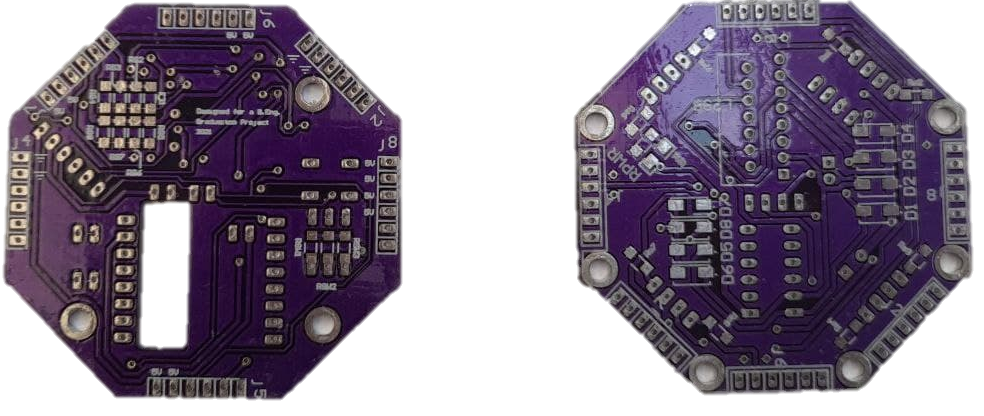
\includegraphics[width=0.9\linewidth]{figs/15/fig15_2}
	\caption{المنتج النهائي بعد تصنيع الدارة}
	\label{15:fig:2}
\end{figure}

\subsection{اختبار المنتج}

بعد عمليّة التّصنيع قمنا بعمليّة فحص للدّارات للتأكّد من التّوصيلات باستخدام الأدوات المختلفة. ووجدنا بعد عمليّة الفحص الأوليّة حدوث قصر في الدّارة ناتج عن انقطاع في الأرضي نتيجة القص الزّائد عند الأطراف، حيث أن أرضي الدّارة يتواجد في الأطراف والصّورة أدناه توضّح منطقة حدوث الانقطاع.

\begin{figure}[h]
	\centering
	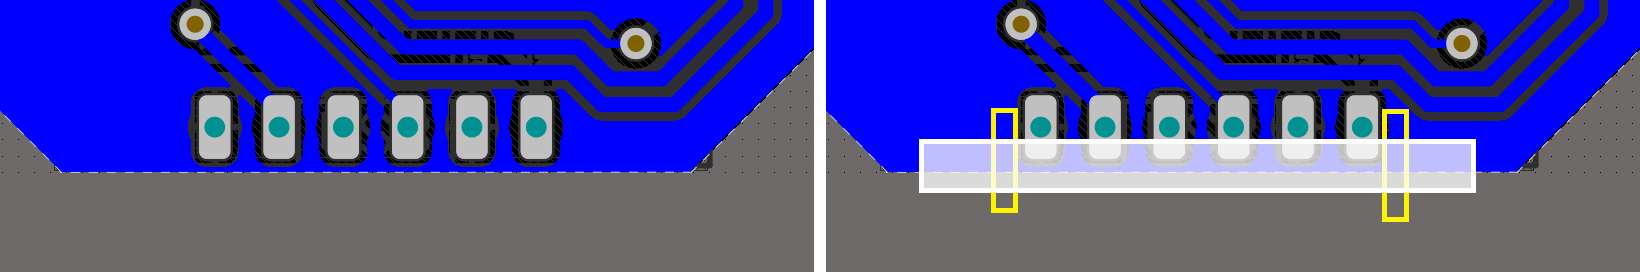
\includegraphics[width=0.9\linewidth]{figs/15/fig15_3}
	\caption{العطب الناتج عن التصنيع}
	\label{15:fig:3}
\end{figure}

لم يقتصر حدوث الانقطاع على منطقة الأرضي بل كان هناك انقطاعات في المناطق الموصلة عند الانتقال من جزء واسع إلى جزء ضيّق ($ necks $). بعد ذلك قمنا بإحصاء أماكن حدوث هذه المشكلة ووجدنا وجود انقطاعين في الطّبقة السّفليّة وانقطاعين في الطّبقة العليا وقمنا بوصل جميع المناطق المقطوعة بأسلاك خارجيّة.

\subsection{الجسم الخارجي والتحريك}

تم تصميم جسم الروبوت باستخدام برنامج SoildWorks واعتماد تصميم بسيط صغير الحجم بأبعاد 6×7×6 بشكل مثمن. تُثبت البطارية من الجهة السفلية للجسم ويوجد أماكن مخصصة لتثبيت المحركات والعجلات والمقاطعات الضوئية وتُبت الدراتين فوق الجسم باستخدام أربع براغي. كما هو موضح في الشكل 

 \begin{figure}[htbp]
	\centering
	\includesvg[width=0.85\linewidth]{figs/15/fig15_5}
	\caption{ الهيكل الخارجي للروبوت}
	\label{15:fig:5}
\end{figure}

تم تصنيع الجسم باستخدام تقنية الطباعة ثلاثية الأبعاد من مادة  Polylactic Acid (PLA)مع خصائص طباعة تتلخص في ارتفاع الطبقة 0.16 ملم وسماكة الجدران 0.8 ملم. 
بعد تجريب ثلاث ورشات متوفرة وسهلة الوصول جغرافيا، توصلنا إلى أفضل طباعة بشكل يضمن الجودة المطلوبة ولاسيما في تصنيع العجلات حيث أن أي اختلاف أو عدم انتظام في الثقوب سيؤثر مباشرة على قيم التغذية الراجعة التي سيعتمدها الروبوت لتتبع المسار الناتج. توضح الصورة \ref{15:fig:6} مقارنة بين علجة مثالية وعجلة ذات جودة تصنيع منخفضة.


\begin{figure}[h]
	\centering
	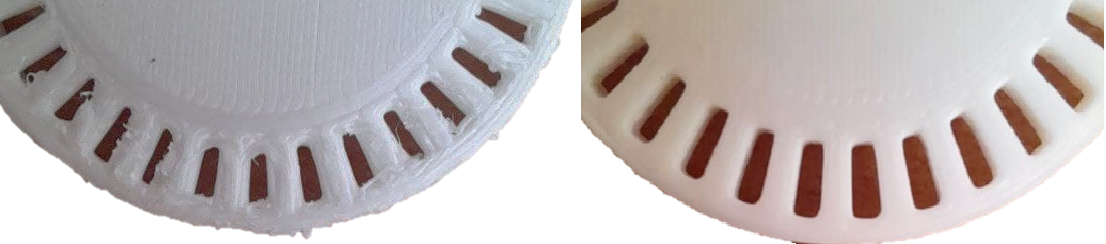
\includegraphics[width=0.9\linewidth]{figs/15/fig15_6}
	\caption{ مثال يوضح مقارنة بين سوء وجودة تصنيع العجلات}
	\label{15:fig:6}
\end{figure}



لضمان حركة مستقرة للروبوت على الأرض ونظراً لخفة وزن الروبوت، قمنا باختيار مادة مناسبة من الكاوتشوك لإحاطة إطارات كل العجلات و زيادة الاحتكاك وبعد التجريب تم تحقيق الغاية المرجوة حيث أن انزلاق العجلات على الأرض كان شبه معدوم. سنعرض النتائج النهائية لتركيب الروبوتات في فصل النتائج.

بالنّسبة لدور العجلات كمسجّلات حركة فكان يجب اختبار دقّة الطّباعة ثلاثيّة الأبعاد في إخراج الشّقوق الموجودة على العجلات، ولاختبار ذلك قمنا بتحريك العجلات بأقصى سرعة يمكن للروبوت السّير بها فكانت استجابة المقاطعات الضّوئيّة لعبور الشقوق عبرها كالتالي (الشكل \ref{15:fig:enc}): 


 \begin{figure}[htbp]
	\centering
	\includesvg[width=0.85\linewidth]{figs/15/fig_enc}
	\caption{استجابة المقاطعات الضّوئيّة}
	\label{15:fig:enc}
\end{figure}

\begin{figure}
	\centering
	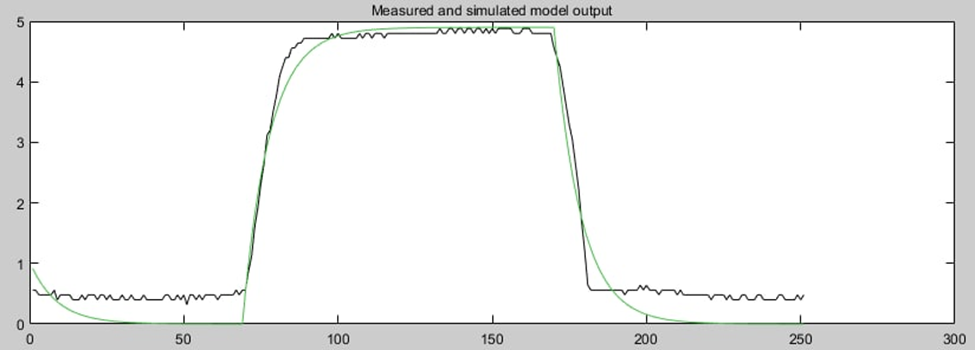
\includegraphics[width=0.9\linewidth]{figs/15/fig15_enc2}
	\caption{التقريب إلى نظام درجة أولى}
	\label{fig:fig15enc2}
\end{figure}

أمّا الخطوة التّالية فكانت اختبار استجابة الـ AVR للمقاطعات الضّوئيّة، وكما نلاحظ من قراءة الاستجابة الموضّحة في الشّكل \ref{fig:fig15enc3} وجود تاخير بسيط في استجابة الـ AVR.

\begin{figure}
	\centering
	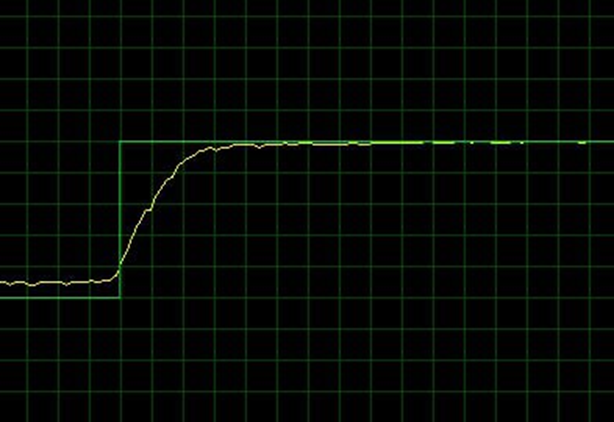
\includegraphics[width=0.7\linewidth]{figs/15/fig15_enc3}
	\caption{محاكاةاستجابة الـ AVR للمقاطعة الضّوئيّة}
	\label{fig:fig15enc3}
\end{figure}

ولتحسين قراءة المقاطعات الضّوئيّة قمنا بتصميم encoder وتصنيعه للحصول على حواف شقوق حادّة ومن ثمّ إطباقه على شقوق العجلات للحصول على أفضل استجابة ممكنة.

\begin{figure}
	\centering
	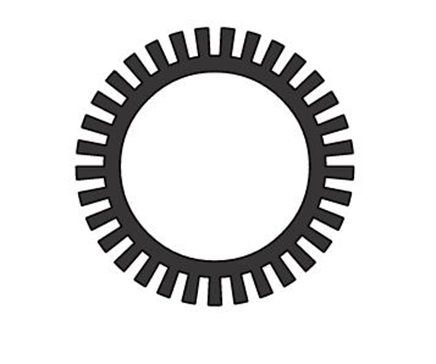
\includegraphics[width=0.5\linewidth]{figs/15/fig15_enc4}
	\caption{طبقة بلاستيكية لتحسن قراءة المقطعات}
	\label{fig:fig15enc4}
\end{figure}
